% floats/figures.tex
% ----------------------------------------------------------------------

\emph{See to-do notes on Figure \ref{fig:locmap}
    \irina{include all geographic names}
    \arjen{elevation scale white-end confused with glaciers}
    \arjen{remove Arctic circle and miles scale}
    \arjen{use CIS, LIS and IIS for ice sheet names}
    \arjen{use N, S, E and W instead of minus, add 75\degree N label}
}

% fig:locmap
\begin{figure}[t]
	\vspace*{2mm}
	\begin{center}
		\includegraphics[width=8cm]{cordillera-climate-locmap}
	\end{center}
	\caption{Shaded relief map of northern North America with the extent of the Cordilleran (CIS), Laurentide (LIS) and Innuitian (IIS) ice sheets at 14\,$^{14}$C\,ka\,BP (16.8\,cal\,ka\,BP) \citep{dyke-2004}. The background map consists of ETOPO1 \citep{data:etopo1} and Natural Earth Data \citep{data:naturalearth}. Assembled with GRASS~GIS \citep{soft:grass} and Inkscape \citep{web:inkscape}}
	\label{fig:locmap}
\end{figure}

% fig:topo
\begin{figure*}[t]
	\vspace*{2mm}
	\begin{center}
		\includegraphics[width=13cm]{cordillera-climate-topo}
	\end{center}
	\caption{Topography maps from CFSR (Climate System Forecast Reanalysis), ERA-Interim reanalysis, NARR (North American Regional Reanalysis), and NCEP/NCAR reanalysis data used as a reference for temperature lapse-rate corrections, and topography map from ETOPO1 used as basal topography. Drawn using Matplotlib \citep{soft:mpl}.}
	\label{fig:topo}
\end{figure*}

% fig:temp
\begin{figure*}[t]
	\vspace*{2mm}
	\begin{center}
		\includegraphics[width=13cm]{cordillera-climate-temp}
	\end{center}
	\caption{Summer (JJA) and winter (DJF) temperature maps from CFSR (Climate System Forecast Reanalysis), ERA-Interim reanalysis, NARR (North American Regional Reanalysis), and NCEP/NCAR reanalysis climatologies. Drawn using Matplotlib \citep{soft:mpl}.}
	\label{fig:temp}
\end{figure*}

% fig:prec
\begin{figure*}[t]
	\vspace*{2mm}
	\begin{center}
		\includegraphics[width=13cm]{cordillera-climate-prec}
	\end{center}
	\caption{Summer (JJA) and winter (DJF) precipitation maps from CFSR (Climate System Forecast Reanalysis), ERA-Interim reanalysis, NARR (North American Regional Reanalysis), and NCEP/NCAR reanalysis climatologies. Drawn using Matplotlib \citep{soft:mpl}.}
	\label{fig:prec}
\end{figure*}

% fig:cool05
\begin{figure*}[t]
	\vspace*{2mm}
	\begin{center}
		\includegraphics[width=13cm]{cordillera-climate-cool05}
	\end{center}
	\caption{Ice surface topography (black contours every 1000\,m) and velocity (\unit{m\,yr^{-1}}) after 10\,kyr under a climate 5\,\unit{\degree C} colder than present for each climate forcing. Drawn using Matplotlib \citep{soft:mpl}.}
	\label{fig:cool05}
\end{figure*}

% fig:extent
\begin{figure*}[t]
	\vspace*{2mm}
	\begin{center}
		\includegraphics[width=13cm]{cordillera-climate-extent}
	\end{center}
	\caption{Extent of ice cover after 10\,kyr as a function of applied temperature offsets for each climate forcing. Drawn using Matplotlib \citep{soft:mpl}.}
	\label{fig:extent}
\end{figure*}

% fig:ivolarea
\begin{figure}[t]
	\vspace*{2mm}
	\begin{center}
		\includegraphics[width=9cm]{cordillera-climate-ivolarea}
	\end{center}
	\caption{Total ice volume and glaciated area after 10\,kyr as a function of temperature offset and climate forcing. Drawn using Matplotlib \citep{soft:mpl}.}
	\label{fig:ivolarea}
\end{figure}

% fig:best
\begin{figure*}[t]
	\vspace*{2mm}
	\begin{center}
		\includegraphics[width=13cm]{cordillera-climate-best}
	\end{center}
	\caption{Ice surface topography (black contours every 1000\,m) after 10\,kyr using temperature offsets that lead to similar areas of ice cover for each climate forcing. 14\,$^{14}$C\,ka\,BP (16.8\,cal\,ka\,BP) ice margin (blue line) from \citet{dyke-2004}. Drawn using Matplotlib \citep{soft:mpl}.}
	\label{fig:best}
\end{figure*}

% fig:oroprecip
\begin{figure}[t]
	\vspace*{2mm}
	\begin{center}
		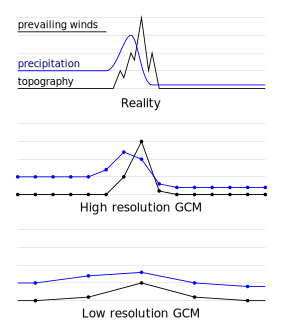
\includegraphics[width=8cm]{cordillera-climate-oroprecip}
	\end{center}
	\caption{Schematic representation of the orographic precipitation effect over the Coast Mountains. In a GCM of lower resolution, the precipitation peak appear smoother and the precipitation shadow is not as pronounced. Drawn using Inkscape \citep{web:inkscape}.}
	\label{fig:oroprecip}
\end{figure}
